\documentclass[12pt,letterpaper]{article}
\usepackage{fullpage}
\usepackage[top=1.5cm, bottom=1.5cm, left=1.5cm, right=1.5cm]{geometry}
\usepackage{amsmath,amsthm,amsfonts,amssymb,amscd}
\usepackage{lastpage}
\usepackage{enumerate}
\usepackage{fancyhdr}
\usepackage{mathrsfs}
\usepackage[dvipsname]{xcolor}
\usepackage{graphicx}
\usepackage{listings}
\usepackage{enumitem} 
\usepackage{hyperref}
\usepackage{caption}
\usepackage{mathtools}
\usepackage{float}
\usepackage{booktabs}
\usepackage{titlesec}
\usepackage{fancyhdr}

\titleformat*{\subsubsection}{\normalfont}
\restylefloat{table}

% \usepackage[document]{ragged2e}
\usepackage{subcaption}
\usepackage{float}
\usepackage{csvsimple}
\usepackage{filecontents}
\usepackage{pgfplotstable,booktabs}


\definecolor{dkgreen}{rgb}{0,0.6,0}
\definecolor{gray}{rgb}{0.5,0.5,0.5}
\definecolor{mauve}{rgb}{0.58,0,0.82}
\definecolor{light-gray}{gray}{0.95}

\newcommand{\code}[1]{\colorbox{light-gray}{\texttt{#1}}}

\lstset{
  language=R,
  aboveskip=3mm,
  frame=single,
  belowskip=3mm,
  showstringspaces=false,
  columns=flexible,
  basicstyle={\small\ttfamily},
  numbers=none,
  numberstyle=\tiny\color{gray},
  keywordstyle=\color{blue},
  commentstyle=\color{dkgreen},
  stringstyle=\color{mauve},
  breaklines=true,
  breakatwhitespace=true,
  tabsize=3,
  numbers=left,
  stepnumber=1
}

\title{\textbf{Machine Problem 2 in STAT 123}}
\date{2020, December 4}
\author{Bascug, Ethan Job \\Dy, Alwyn \\ Fortaleza, Camelle Faye \\Portuito, Rey Joseph}

% \pagestyle{fancy}
% \rhead{\thesection}


\begin{document}
    \maketitle

    \section*{Problem 1}
    \paragraph*{Let $X$ be a discrete random variable with distribution $f$, and let $a<b$. Sketch the distribution functions of the 'truncated' random variables $Y$ and $Z$ given by}

    \begin{equation*}
      Y = \left\{
        \begin{array}{ll}
            a & \quad \mbox{if } X < a, \\
            X & \quad \mbox{if } a \leqslant X \leqslant b,\\
            b & \quad \mbox{if } X>b
        \end{array}
      \right. \hspace*{0.5cm}
      Z = \left\{
        \begin{array}{ll}
            X & \quad \mbox{if } \lvert X \rvert \leqslant a, \\
            0 & \quad \mbox{if } \lvert X \rvert  > b
        \end{array}
      \right.
    \end{equation*}
    \paragraph*{Indicate how these distributions functions behave as $a\rightarrow -\infty$, $b \rightarrow \infty$.}

    \begin{enumerate}[label=\Alph*]
      \vspace*{0.5cm}
      \item \textbf{Algorithm and R Code}\\
        Since $X$ is a discrete random variable, we can generate $n$ random values for $X$. Additionally, $a$ and $b$ can be any arbitrary numbers where $a < b$. 

        \vspace*{0.5cm}
        For the 'truncated' random variable $Y$,
        \begin{enumerate}[label=\arabic*.]
          \item Traverse the entirety of $X$ (from 1 to $n$) and do the following truncation to all its elements (i.e. change the value if it satisfies the condition):
            \begin{enumerate}[label=1.\arabic*.]
              \item if the value is less than $a$, change the value to $a$,
              \item else, if the value is greater than $b$, change it to $b$
              \item otherwise, do nothing
            \end{enumerate}
          \item Return the truncated random variable.
        \end{enumerate}

        \vspace*{0.5cm}
        For the 'truncated' random variable $Z$,
        \begin{enumerate}[label=\arabic*.]
          \item Traverse the entirety of $X$ (from 1 to $n$) and do the following truncation to all its elements (i.e. change the value if it satisfies the condition):
            \begin{enumerate}[label=1.\arabic*.]
              \item if the absolute value of $X$ is greater than $b$, change the value to 0,
              \item otherwise, do nothing
            \end{enumerate}
          \item Return the truncated random variable.
        \end{enumerate}
        \newpage
        \begin{lstlisting}[title=\footnotesize Code 1.1: Function for the truncation of $Y$ and $Z$]
YTruncation <- function(x, a, b){
  for (i in 1:length(x)){
    if (x[i] < a)           x[i] <- a
    else if (x[i] > b)      x[i] <- b
  }
  return (x)
}

ZTruncation <- function (x,b){
  for (i in 1:length(x)){
    if (abs(x[i]) > b)      x[i] <- 0
  }
  return (x)
}
        \end{lstlisting}
        \vspace*{0.5cm}
       \item \textbf{Simulation and Analysis} 
       
       For this simulation, we assume $X$ has a binomial distribution $f$. Using \code{set.seed(141421356)} (for replication of results), we generate 1000 ($n=1000$) random values for $X$ with a size of 100 and a probability of 0.23, shown in Code 1.2. A histogram of the randomly generated values can be seen in Figure 1.1.
       \begin{lstlisting}[title=\footnotesize Code 1.2: Initialization of $X$]
x <- rbinom(1000,size = 100, prob=0.23)  
       \end{lstlisting}

       \begin{figure*}[h]
          \centering 
          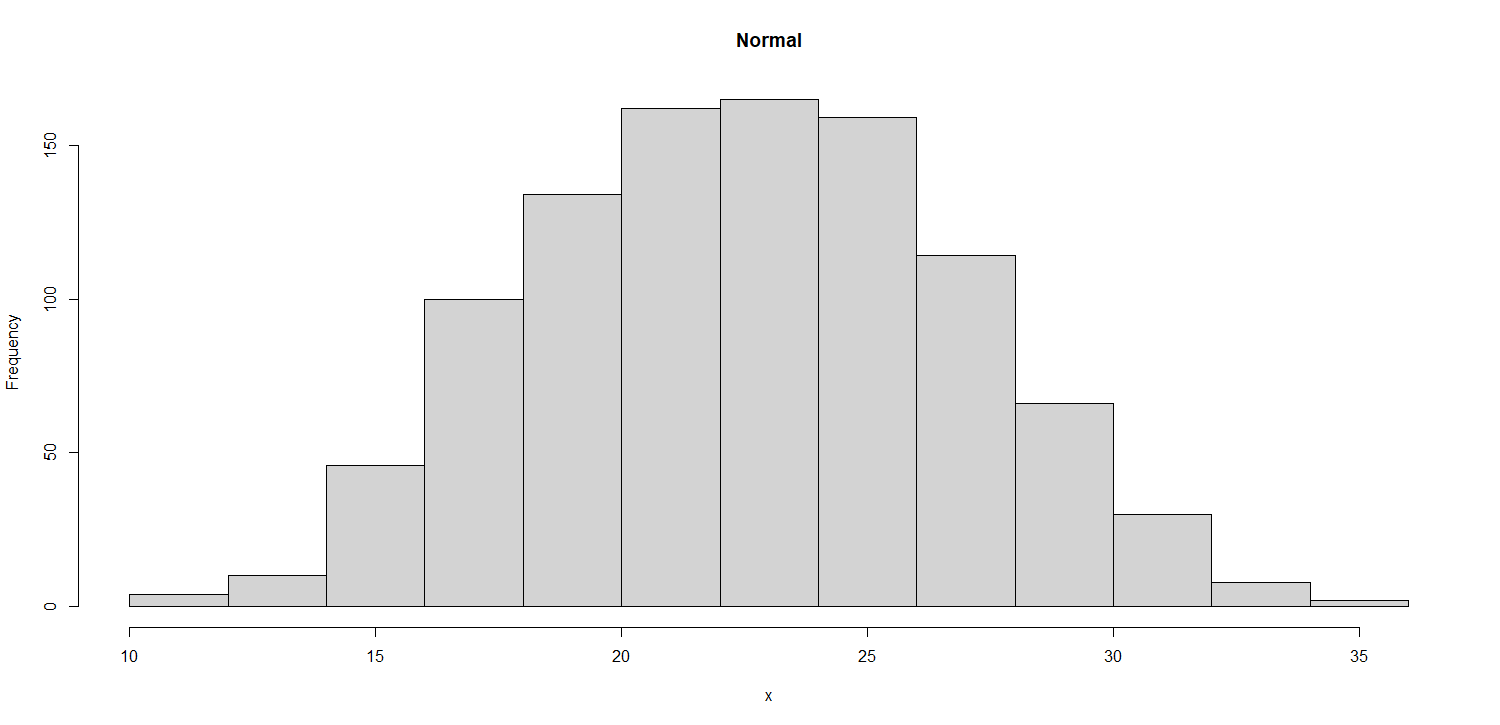
\includegraphics[scale=0.4]{normal.png}
          \caption*{\footnotesize Figure 1.1: Distribution of the randomly generated values for $X$}
       \end{figure*}
       
       \newpage
       Using the values for $a$ and $b$ found in Table 1.1, we truncate $X$ using the truncation functions for $Y$ (below, left column) and $Z$ (below, right column). The values for $a$ and $b$ were chosen such that it starts near the mean of $X$ ($\mu = 23.047$) and grow outward such that $a\rightarrow -\infty$ and $b \rightarrow \infty$.

       \begin{table}[H]\centering
          \footnotesize Table 1.1: Values for $a$ and $b$ used in the truncation functions $Y$ and $Z$

       \vspace*{0.3cm}
          \begin{tabular}{l|lllll} \toprule
            Case  & 1   &  2  &  3  &  4   &  5\\ \midrule
            a     & 22  &  20 &  15 &  10  &  0\\
            b     & 25  &  30 &  35 &  40  &  50\\ \bottomrule
          \end{tabular}
       \end{table}

       \begin{figure}[H]
         \centering 
         \begin{subfigure}[H]{0.49\textwidth}
           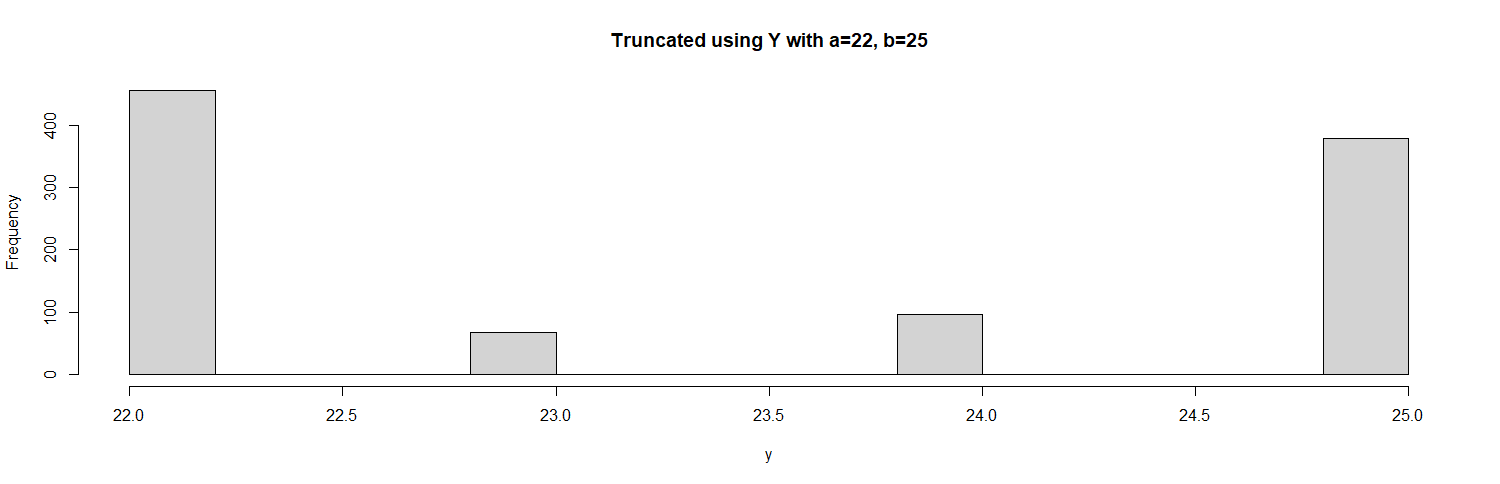
\includegraphics[width=\textwidth]{Y-22-25.png}
            \caption*{\footnotesize Case 1.1: Truncated Y using $a=22$, $b=25$}
         \end{subfigure}
         \begin{subfigure}[H]{0.49\textwidth}
          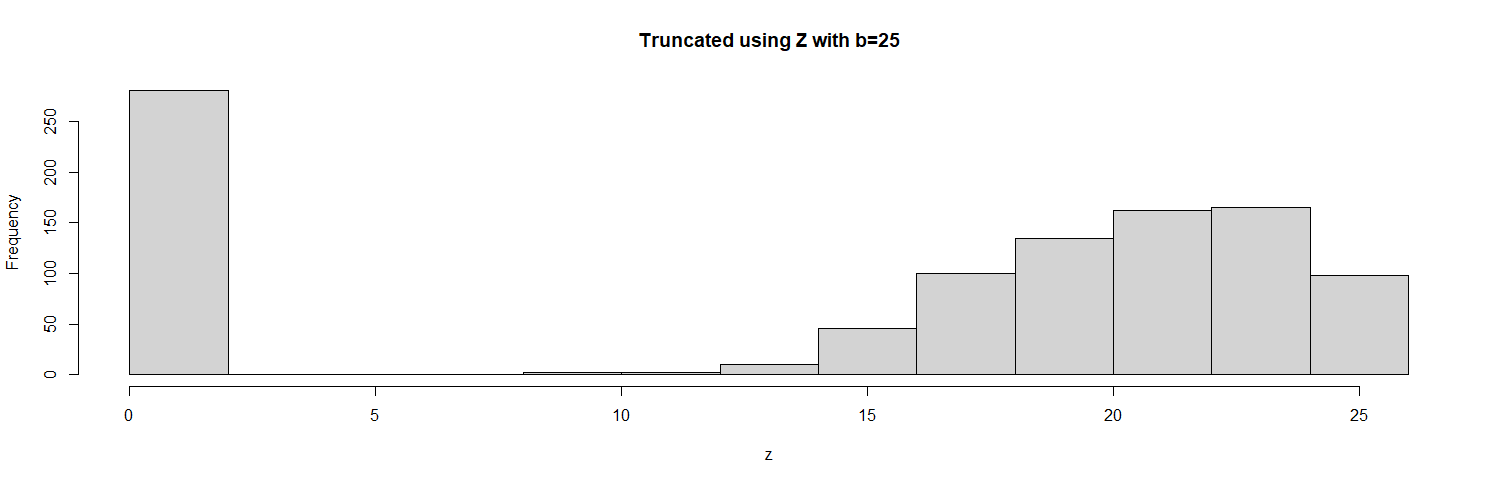
\includegraphics[width=\textwidth]{Z-25.png}
          \caption*{\footnotesize Case 1.2: Truncated Z using $b=25$}
        \end{subfigure}
        \begin{subfigure}[H]{0.49\textwidth}
          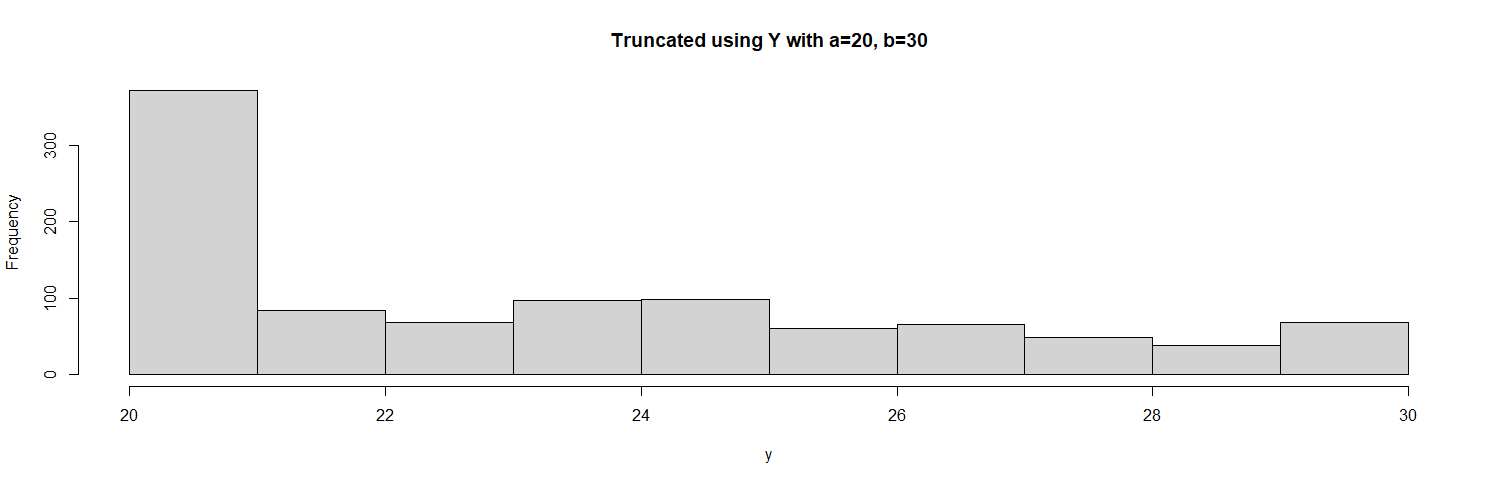
\includegraphics[width=\textwidth]{Y-20-30.png}
          \caption*{\footnotesize Case 2.1: Truncated Y using $a=20$, $b=30$}
        \end{subfigure}
        \begin{subfigure}[H]{0.49\textwidth}
          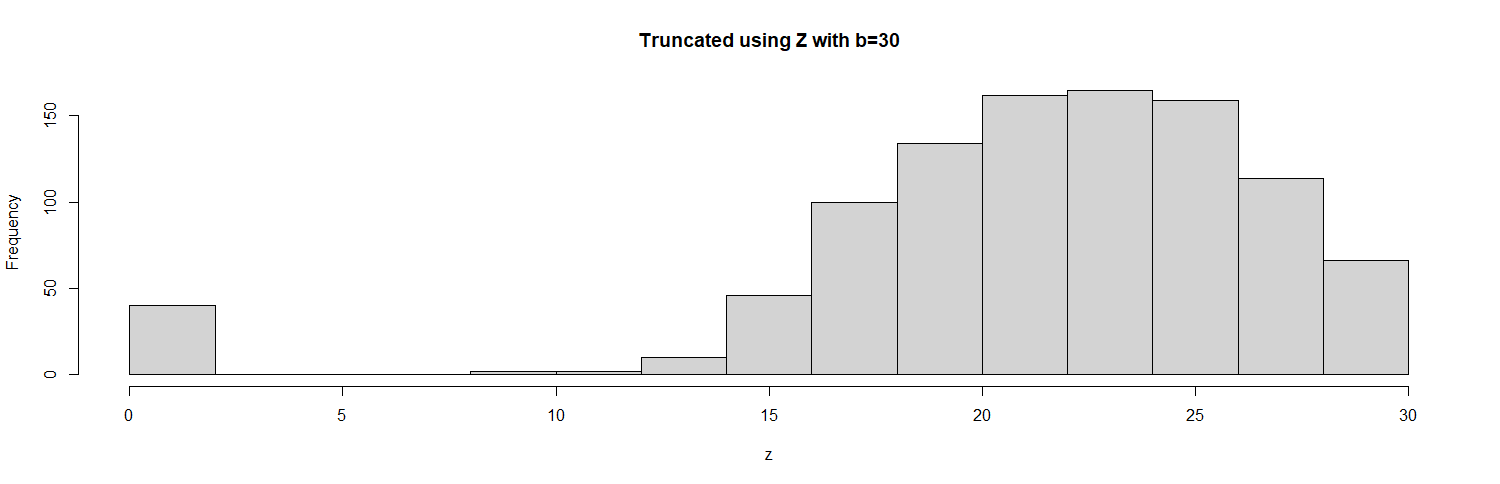
\includegraphics[width=\textwidth]{Z-30.png}
          \caption*{\footnotesize Case 2.2: Truncated Z using $b=30$}
        \end{subfigure}
        \begin{subfigure}[H]{0.49\textwidth}
          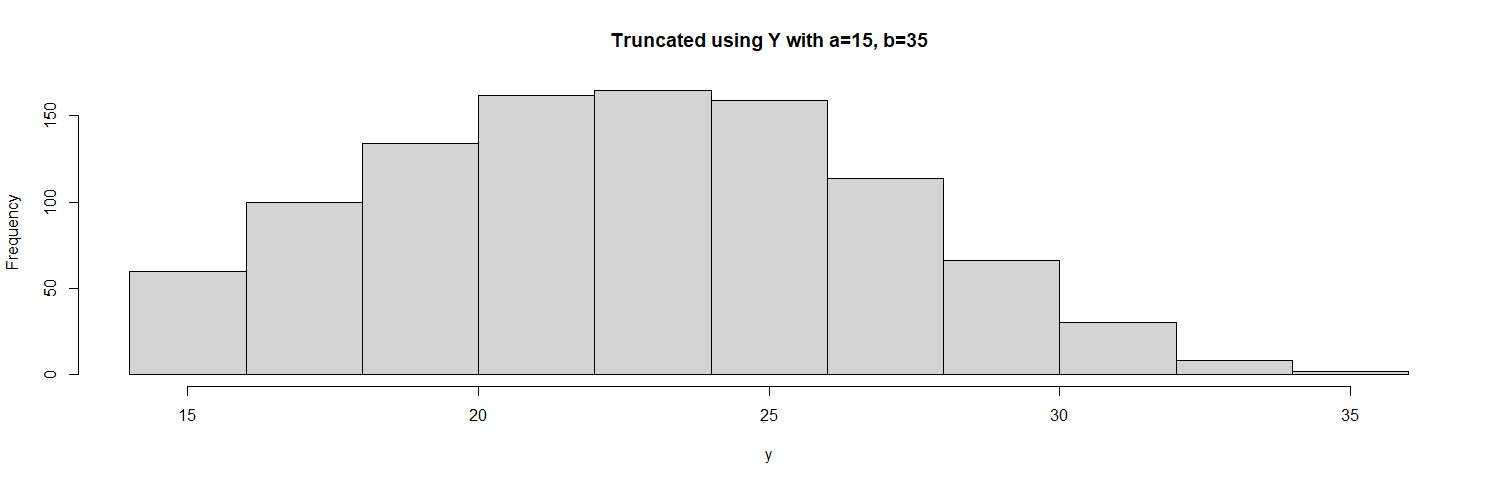
\includegraphics[width=\textwidth]{Y-15-35.png}
          \caption*{\footnotesize Case 3.1: Truncated Y using $a=15$, $b=35$}
        \end{subfigure}
        \begin{subfigure}[H]{0.49\textwidth}
          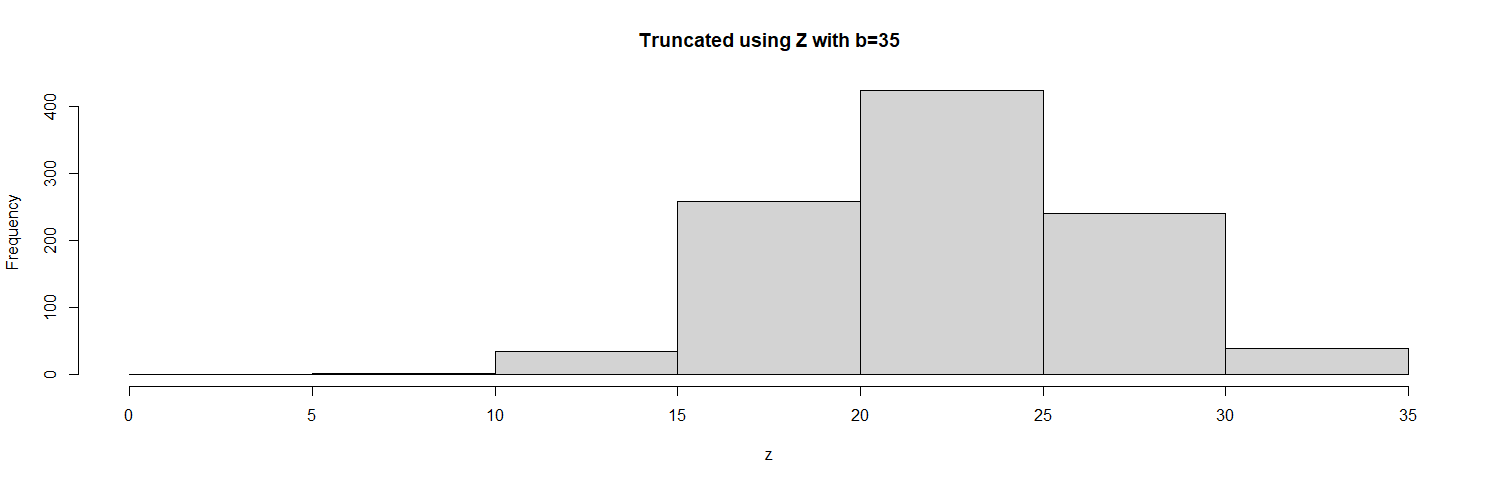
\includegraphics[width=\textwidth]{Z-35.png}
          \caption*{\footnotesize Case 3.2: Truncated Z using $b=35$}
        \end{subfigure}
        \begin{subfigure}[H]{0.49\textwidth}
          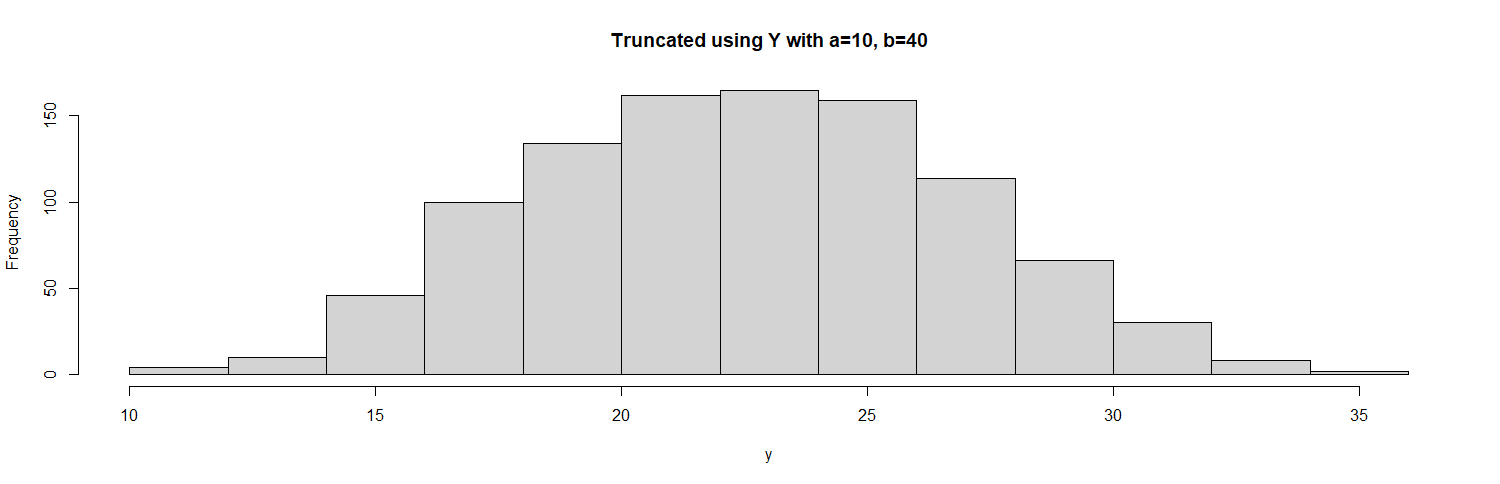
\includegraphics[width=\textwidth]{Y-10-40.png}
          \caption*{\footnotesize Case 4.1: Truncated Y using $a=10$, $b=40$}
        \end{subfigure}
        \begin{subfigure}[H]{0.49\textwidth}
          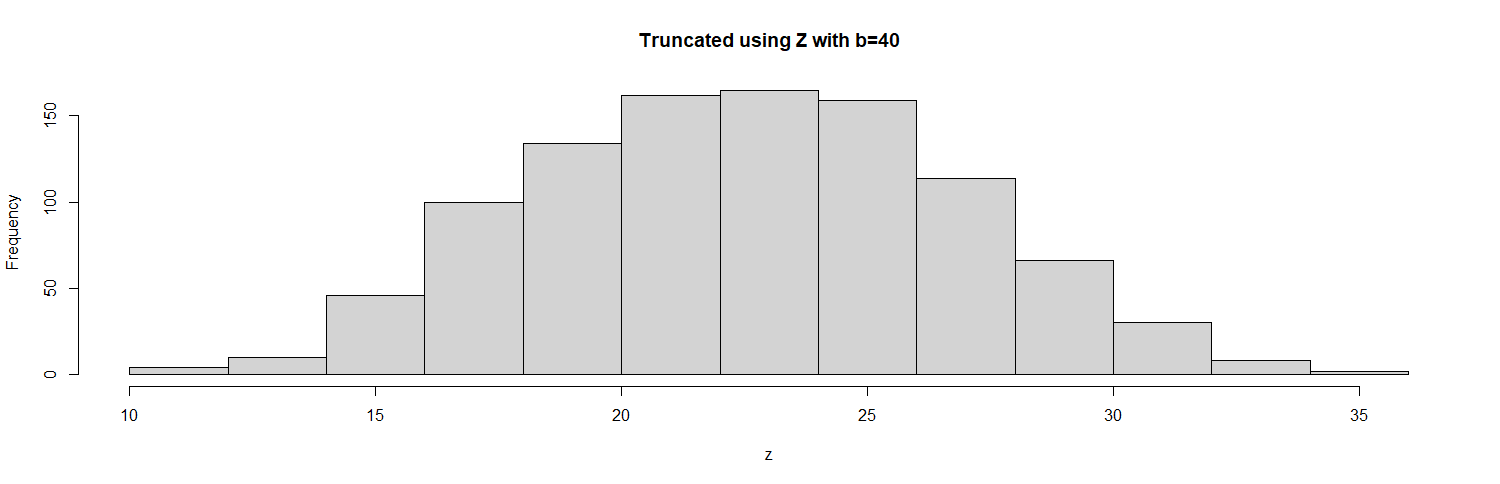
\includegraphics[width=\textwidth]{Z-40.png}
          \caption*{\footnotesize Case 4.2: Truncated Z using $b=40$}
        \end{subfigure}
        \begin{subfigure}[H]{0.49\textwidth}
          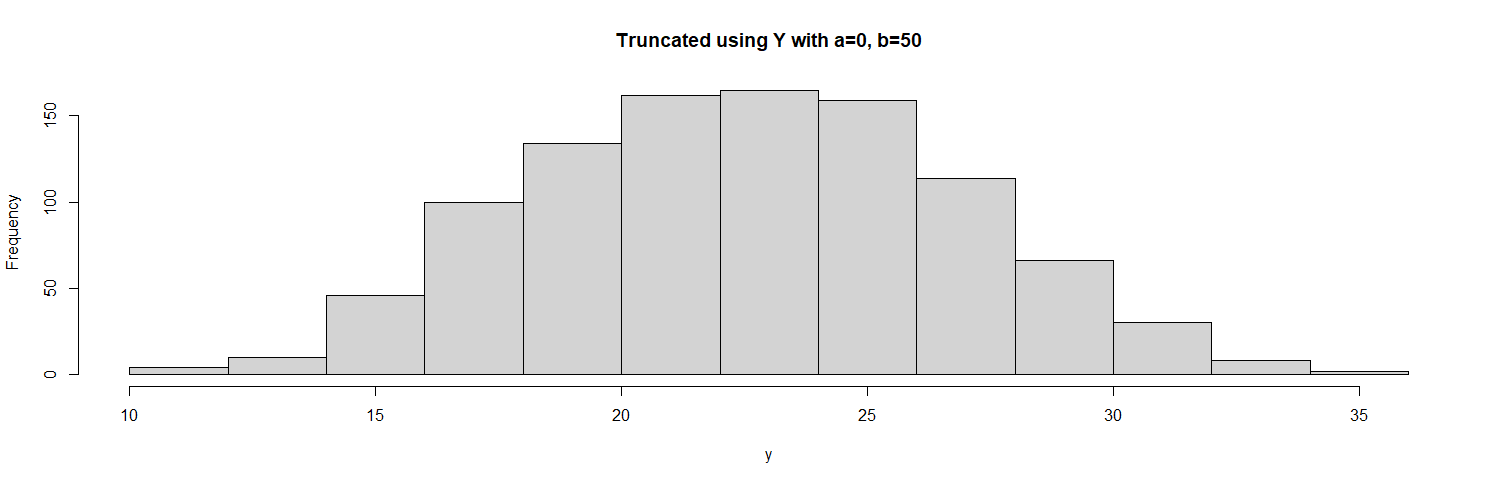
\includegraphics[width=\textwidth]{Y-0-50.png}
          \caption*{\footnotesize Case 5.1: Truncated Y using $a=0$, $b=50$}
        \end{subfigure}
        \begin{subfigure}[H]{0.49\textwidth}
          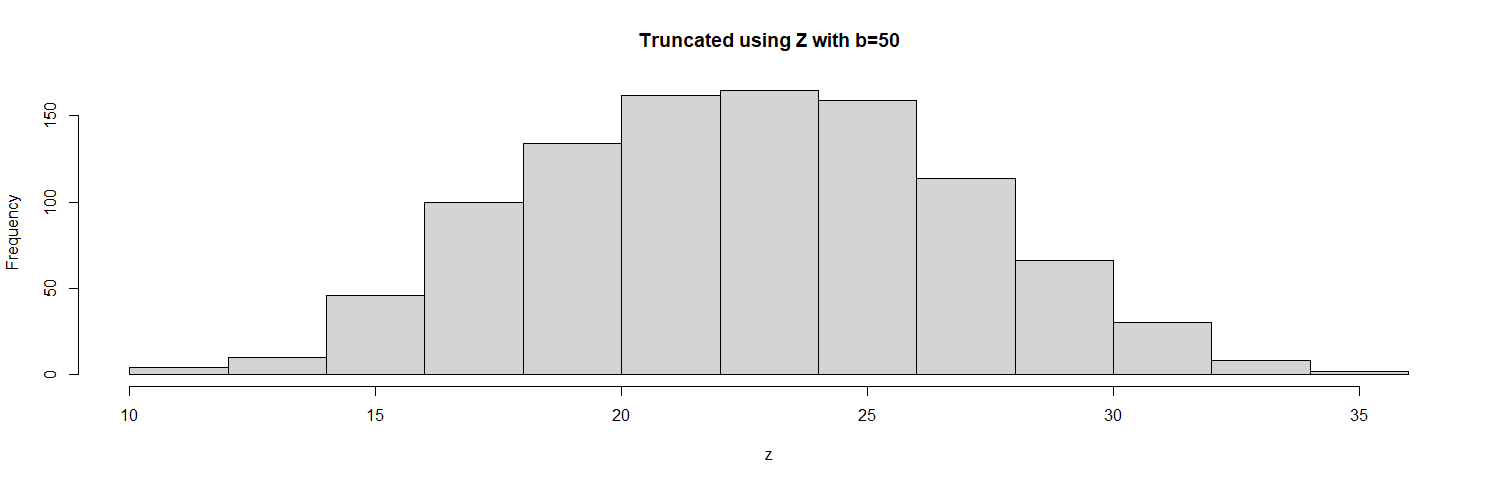
\includegraphics[width=\textwidth]{Z-50.png}
          \caption*{\footnotesize Case 5.2: Truncated Z using $b=50$}
        \end{subfigure}
       \end{figure}
       \vspace{5cm}
       Analyzing the graphs found in the previous page, we can infer that the truncation function $Y$ limits the values for the random variable to be within the interval $[a, b]$. The function prevents the values to exceed beyond the interval by capping the values at the boundaries. Meanwhile the truncation function $Z$ limits the random variable to be within the interval $[-b, b]$ by converting the values that exceeded the interval to 0. 

       Moreover, as $a\rightarrow -\infty$ and $b \rightarrow \infty$, the distribution of the truncated random variables $Y$ and $Z$ becomes similar to $f$, it approaches the original (untruncated) distribution. Beyond certain values, the truncation functions will have no effect to the random variable, as seen in cases 5.1 and 5.2 where $a=0$ and $b=50$.

    \end{enumerate}
    \newpage

    %%%%%%%%%%%%%%%%%%%%%%%%%%%%%%%%%%%%%%%%%%%%%%%%%%%%%%%%%%%%%%%%%%%%%%%%%%%%%%%%

    \section*{Problem 2}

    \paragraph*{Airlines find that each passenger who reserves a seat fails to turn up with probability $q$ independently of the other passengers. So Airline $A$ always sell $n$ tickets for their $n-1$ seat aeroplane while Airline $B$ always sell $2n$ tickets for their $2n-2$ seat aeroplane. Which is more often over-booked?}

    \hspace*{0.5cm} \vspace*{0.5cm}
    \begin{enumerate}[label=\Alph*]
      \item \textbf{Algorithm}
      
        \begin{enumerate}[label=\arabic*.]
          \item Assign values to the given variables.
          \item Use the formula in getting the probability and combination.
          \item Observe the results of both Airlines after you perform the operations.
          \item Identify which Airline is often overbooked.
        \end{enumerate}

      \vspace*{0.5cm}
      \item \textbf{R Code}
      
        \begin{lstlisting}
#Number3

#To solve this problem with ease, we assign values to the given variables:
#Let q be 10% the probability that a passenger did not show up
q<- 0.10
#Let n be 10 the passengers Airline A can hold.
n<- 10
#Let 1-q be the probability of passengers that shows up 

#COMPUTE

Prob_of_Airline_A<- (1-q)^n #Use this formula, (1-q)^n, to get the probability that all 10 passengers shows up.
Prob_of_Airline_A

Prob_of_Airline_B<- (1-q)^(2*n)+.1^1 * .9^19 *factorial(20)/factorial(19)*factorial(1) #Use this formula, (1-q)^(2*n)+.1^1 * .9^19 *(20!/19!*1!) to get the probability of all 20 or 19 passengers shows up.  
Prob_of_Airline_B

#Airline B (0.391747) is often over-booked than Airline A (0.3486784)
        \end{lstlisting}

      \vspace*{0.5cm}
      \item \textbf{Mathematical Calculations}
      
        We assign values to the variables given to the problem, so that we can solve the problem with ease;

        \hspace*{0.5cm} Let $q$ be 0.10, the probability that a passenger did not show up.\\
        \hspace*{0.5cm} Let $n$ be 10, the passengers Airline A can hold.\\
        First,
        \begin{equation*}
          1-q=1-0.10=0.90
        \end{equation*}

        0.90 is the probability that the passenger will show since there is only 0.10 probability that they will not show up. There are 10 passengers that has 0.90 probability of showing up. So, we will use this formula, $(1-q)^n$, to obtain the overbooking probability of Airline A.

        We proceed in computing the probability of Airline A by,
        \begin{equation*}
          P^a = (1-q)^n = 0.90^{10} = 0.34867844
        \end{equation*}

        For Airline B the probability of it to be overbook happens when all 20 passengers show up or when 19 of the20 passengers show up for the 18 seats.

        The probability that all 20 passengers will show up is,
        \begin{equation*}
          (1-q)^n=0.90^{20} = 0.121576655
        \end{equation*}

        The probability that 19 passengers will show up is,
        \begin{equation*}
          (q^1) \times (1-q)^{19} \times 
            \left( {\begin{array}{*{20}c}
               2n  \\
               2n-1  \\
            \end{array}} \right)
             = 0.1^1 \times 0.9^{19} \times 
             \left( {\begin{array}{*{20}c}
              20  \\
              1  \\
           \end{array}} \right)
            = 0.270170344
        \end{equation*}
        
        We considered  "$q^1$" since there is a probability that one passenger will not show up and also, {\footnotesize “$\left( {\begin{array}{c}
          2n  \\
          2n-1  \\
       \end{array}} \right)$”} since it determines the possible combinations of selecting 1 out of 20. 

       To determine the probability of Airline B is by,
       \begin{align*}
         P^b &= (1-9)^n + (q^1) \times (1-q)^{19} \times 
         \left( {\begin{array}{*{20}c}
          2n  \\
          2n-1  \\
          \end{array}} \right)\\
          &= 0. 121576655 + 0 .270170344\\
          &= 0.391746998
       \end{align*}

       $\therefore$ Airline B (0.391746998) is often overbooked than Airline A (0.34867844).
    \end{enumerate}

    \newpage

%%%%%%%%%%%%%%%%%%%%%%%%%%%%%%%%%%%%%%%%%%%%%%%%%%%%%%%%%%%%%%%%%%%%%%%%%%%%%%%%%%%%

    \section*{Problem 3}
       
    \paragraph*{Paul rolls $6n$ dice once; he needs at least $n$ sixes. Yves rolls $6(n + 1)$ dice; he needs at least $n + 1$ sixes. Simulate this game and determine who among Paul or Yves is more likely to obtain the number of sixes he needs.}
    \hspace*{1cm}
    \vspace*{0.5cm}
    \begin{enumerate}[label=\Alph*]

      \item \textbf{Algorithm and R Code}
        \begin{lstlisting}[title=\footnotesize Code 3.1: The Entire Code]
number_3 = function(n){
  Paul = 6 * n
  Yves = 6 * (n + 1)
  Paul_roll = sample(1:6, Paul, replace = T)
  Yves_roll = sample(1:6, Yves, replace = T)
  
  p = table(Paul_roll)
  y = table(Yves_roll)
  
  Paul_sixes = p[names(p) == 6]
  Yves_sixes = y[names(y) == 6]
  
  print(paste("Number of Rolls (Paul):",Paul))
  print(paste("Number of Rolls (Yves):",Yves))
  
  print(paste("Number of Sixes (Paul):",Paul_sixes))
  print(paste("Number of sixes (Yves):",Yves_sixes))
  
  probP_Paul = Paul_sixes/Paul
  probP_Yves = Yves_sixes/Yves
  
  print(paste("Success (Paul):", probP_Paul))
  print(paste("Fail (Paul):", probQ_Paul))A
  print(paste("Success (Yves):", probP_Yves))
  print(paste("Fail (Yves):", probQ_Yves))
  
  
  prob_Paul = 1 - pbinom(n - 1, size = Paul, prob = probP_Paul)
  prob_Yves = 1 - pbinom(n, size = Yves, prob = probP_Yves)
  
  print(prob_Paul)
  print(prob_Yves)
}
        \end{lstlisting}
      
        \newpage
        To simulate the problem, we have created a function for this named \code{number\_3} with the parameters of \code{n}. First, it initializes the number of rolls Paul and Yves will have. Then simulate those roles based on the number of rolls Paul and Yves have which will be named \code{Paul\_roll} and \code{Yves\_roll}, respectively. This can be found on Code 3.2: Initialization.

          \begin{lstlisting}[title=\footnotesize Code 3.2: Initialization]
number_3 = function(n){
  Paul = 6 * n
  Yves = 6 * (n + 1)
  Paul_roll = sample(1:6, Paul, replace = T)
  Yves_roll = sample(1:6, Yves, replace = T)
          \end{lstlisting}

        For the next part of the code, the \code{p} and \code{y} corresponds to Paul and Yves where the simulated rolls are made into a table where the value of each roll is counted. An example would be Paul’s roll has 10 sixes, 25 three’s, 30 fours and so on. \code{Paul\_sixes} and \code{Yves\_sixes} are the variables that isolates the number of sixes only for both players. This can be found in Code 3.3: Counting

          \begin{lstlisting}[title=\footnotesize Code 3.3: Counting]
  p = table(Paul_roll)
  y = table(Yves_roll)

  Paul_sixes = p[names(p) == 6]
  Yves_sixes = y[names(y) == 6]
          \end{lstlisting}

        The variables \code{probP\_Paul} and \code{probP\_Yves} stands for the probability of success of having rolled a 6 for Paul and Yves. This computes the number of sixes both players has divided the number of rolls they made. This can be found in Code 3.4: Success and Failure

          \begin{lstlisting}[title=\footnotesize Code 3.4: Success and Failure]
  probP_Paul = Paul_sixes/Paul
  probP_Yves = Yves_sixes/Yves
          \end{lstlisting}

        The variables \code{prob\_Paul} and \code{prob\_Yves} indicates the probability of Paul obtaining $n$ 6 sixes and Yves obtaining $n + 1$ sixes. In this section, we used the function \code{pbinom()} where it computes the $P(X \leq x)$ using the binomial distribution. Since we are looking for $P(X \geq x)$, we used the formula $P(X > x) = 1 - P(X \leq x)$.

          \begin{lstlisting}[title=\footnotesize Code 3.5: Probability]
  prob_Paul = 1 - pbinom(n - 1, size = Paul, prob = probP_Paul)
  prob_Yves = 1 - pbinom(n, size = Yves, prob = probP_Yves) 
          \end{lstlisting}
        
        \newpage
      \item \textbf{Simulation}  
        
        Given the varied number of simulations that was made, different probabilities was inferred from the function. Since the probabilities are too varied to draw a conclusion, the average will be taken from these results.

        \begin{figure*}[h]
          \centering
          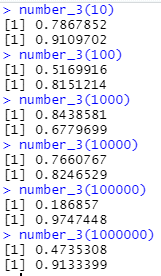
\includegraphics{fig3.1.png}
          \caption*{\footnotesize Figure 3.1: Results of the simulation}
        \end{figure*}

        % \vspace*{0.5cm}
        \begin{align*}
          \mbox{Let} p&=\mbox{probability of Paul getting $n$ ammount/s of six}\\
          \mbox{Let} y&=\mbox{probability of Yves getting $n+1$ ammount/s of six}\\\\
          p&=\frac{0.7868+0.5170+0.8439+0.7661+0.1869+0.4735}{6}\\
          &=0.5957=59.57\%\\\\
          y&=\frac{0.9110+0.8151+0.6780+0.8247+0.9747+0.9133}{6}\\
          &=0.8528=85.28\%
        \end{align*}

        \item \textbf{Conclusion}
        
        Given that Paul has $6n$ rolls and must have $n$ number of six, while Yves has $6(n + 1)$ rolls and must have $n+1$ number of sixes. Using the function coded for number 3, which simulated the situation. Yves has a 85.28\% chance to have $n + 1$ sixes given that he has $6(n + 1)$ rolls, while Paul has only 59.57\% chance to have $n$ sixes given that he has $6n$ rolls. Which makes Yves more likely to have $n + 1$ sixes, rather than Paul having $n$ sixes.
    \end{enumerate}

    \newpage
%%%%%%%%%%%%%%%%%%%%%%%%%%%%%%%%%%%%%%%%%%%%%%%%%%%%%%%%%%%%%%%%%%%%%%%%%%%%%%%%%%%%%%%%%%%%

    \section*{Problem 4}
    \paragraph*{Each member of a group of n players rolls a die.}
    \begin{enumerate}[label=(\alph*)]
      \item For any pair of players who throw the same number, the group scores 1 point. Find the mean and variance of the total score of the group.
      \item Find the mean and variance of the total score if any pair of players who throw the same number scores that number.
    \end{enumerate}




    \newpage

    %%%%%%%%%%%%%%%%%%%%%%%%%%%%%%%%%%%%%%%%%%%%%%%%%%%%%%%%%%%%%%%%%%%%%%%%%%%

    \section*{Problem 5}
    \paragraph*{Every package of some intrinsically dull commodity includes a small and exciting plastic object. There are \textit{k} different types of object, and each package is equally likely to contain any given type. You buy one package each day.}
    
    \begin{enumerate}[label=(\alph*)]
        \item Find the mean number of days which elapse between the acquisitions of the $n^{th}$ new type of object and the $(n+1)^{th}$ new type.
        \item Find the mean number of days which elapse before you have a full set of \textit{k} objects.
    \end{enumerate}
    \vspace*{0.5cm}
    \begin{enumerate}[label=\Alph*]
        \item \textbf{Algorithm and R Code}\\
        To solve for \textit{(a)}, we create a counter that counts the number of days elapsed since receiving a new type of object. We reset it to 0 once we receive a new type. Additionally, since the algorithm has basically finished its function once we receive all types of object, we terminate it once we reach that point. Moreover, to calculate the mean number of elapsed days, we disregard the first day of receiving the object since its value is 0. 
        \begin{enumerate}[label=\arabic*.]
            \item Input \textit{k}, the number of different types of object. Since a descriptive information of the types of object is not necessary, we represent all the different types using integer values from 1 to k.
            \item Randomly choose an object, from 1 to k.
            \item Check if the object has already been received previously. If it hasn't, 
            \begin{enumerate}[label=3.\arabic*]
                \item add it to the list of received objects, 
                \item record the days since a new type of object is received, and
                \item reset the elapsed days counter. 
            \end{enumerate}
                In this way, we can ascertain that all types of objects are received and the days elapsed are recorded. 
            \item Increment the elapsed days counter.
            \item If there are still objects that haven't been received, repeat steps 2 to 5 until all types of objects are received. 
            \item Return the calculated mean of the elapsed days and the total number of days. We acquire the total number of days by summing all elapsed days and adding 1 (this is to account for the first day of receiving the object).
        \end{enumerate}
        \newpage
        \begin{lstlisting}[title=\footnotesize Code 5.1: \code{nicePackage} function]
nicePackage <- function(k){
  set.seed(6626068) # allow for replication of results
  recievedObj <- c() # records received object
  daysPassed <- c() # vector for storing elapsed days until receiving new object
  elapsed <- 0 # elapsed days counter
  
  while (length(recievedObj) < k) { # loops until a complete set is reached
    obj <- ceiling(runif(1, min=0, max=k))
    
    flag <- 0 # determines if obj is already received
    for (j in recievedObj){
      if (j == obj){
        flag <- 1
        break
      } 
    }
    if (flag == 0){ # if received object is new,  
      recievedObj <- c(recievedObj, obj) # add to receivedObj,
      if (elapsed != 0)       
        daysPassed <- c(daysPassed, elapsed) # records elapsed days
      elapsed <- 0 # reset counter
    }
    
    elapsed <- elapsed + 1 
  }

  # returns the mean number of elapsed days and total days to have a full set
  return (c(mean(daysPassed), sum(daysPassed+1)))
}
        \end{lstlisting}

        To solve for (b), we utilize the second element of \code{nicePackage}'s return value (i.e. the total number of days). And since this requires multiple iterations of the first algorithm, we create a new function.    

        \begin{enumerate}[label=\arabic*.]
            \item Input \textit{k}, the number of different types of object, and the number of iterations, \textit{n}.
            \item Iterate \code{nicePackage} \textit{n} times and record the total number of days to receive all the types of objects.
            \item Return the mean number of days.
        \end{enumerate}

        \begin{lstlisting}[title=\footnotesize Code 5.2: \code{manyNicePackages} function]
manyNicePackages <- function(k, n) {
  set.seed(981) # allow for replication of results
  totalDays <- c()
  
  for (i in 1:n)
    totalDays <- c(totalDays, nicePackage(k)[2])
  
  return (mean(totalDays))
}
        \end{lstlisting}

        % \vspace*{0.5cm} 
        \item \textbf{Simulation and Analysis}

        Running the \code{nicePackage} function above with $k=101$ (101 unique objects), we get a mean of 5.81 days. Additionally, a k of only 13 yields a mean of 2.92 days. A visualization of the number of days passed before getting the $n+1^{th}$ object can be seen in Figure 5.2 and Figure 5.3.
        \begin{figure}[H]
          \centering

          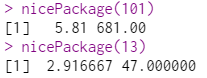
\includegraphics[scale=0.7]{nicePackage.png}
          \caption*{\footnotesize Figure 5.1: RStudio output for the \code{nicePackage} simulation}
          \includegraphics*[scale=0.4]{fig5.1.png}
          \caption*{\footnotesize Figure 5.2: \code{nicePackage} with $k=101$}

          \includegraphics*[scale=0.4]{fig5.2.png}
          \caption*{\footnotesize Figure 5.3: \code{nicePackage} with $k=13$}
          
        \end{figure}

        Moreover, running the \code{manyNicePackages} function with $k=101$ (101 unique objects), $n=50$ (50 iterations of the \code{nicePackage} function), and removing the \code{set.seed(6626068)} in the \code{nicePackage} function, we get a mean of 622.08 days. While a $k=13$ and $n=50$ results to a mean of 55.36 days. It is important to note that the values for $k$ and $n$ were chosen such that the simulation covers from a relatively small to a relatively large number of objects.
        \vspace*{0.8cm}
        \begin{figure*}[h]
          \centering
          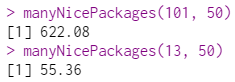
\includegraphics[scale=0.7]{manyNicePackage.png}
          \caption*{\footnotesize Figure 5.4: RStudio output for the \code{manyNicePackages} simulation}
        \end{figure*}

    \end{enumerate}
    
    
\end{document}